\begin{activite}[Multiple, diviseur]

\begin{partie}[Le jeu de Juniper Green]
Règle du jeu : Ce jeu se joue à deux (ou plus) avec \textbf{uniquement} les nombres entiers de 1 à 40.

\begin{itemize}
 \item Le premier joueur choisit un nombre entier.
 \item Le deuxième joueur doit alors en choisir un autre qui doit être soit multiple, soit diviseur de ce premier nombre.
 \item Le joueur suivant en choisit encore un autre qui doit être soit multiple, soit diviseur du second nombre. Et ainsi de suite, chaque nombre ne pouvant servir qu'une seule fois ! 
 \item Le dernier joueur qui a pu choisir un nombre a gagné ! 
 \end{itemize}
 
\begin{enumerate}
 \item Jouez à ce jeu, en alternant le premier joueur ;
 \item Le premier joueur prend 40 comme nombre de départ. Quelle est la liste des nombres possibles pour le second joueur ? Même question avec 17 ; 9 et 23 ;
 \item Dans une partie à deux joueurs, quel nombre peut choisir le premier joueur pour être sûr de l'emporter (s'il joue bien !) ? Trouve toutes les possibilités.
 \end{enumerate}
\end{partie}


\begin{partie}[Liste des diviseurs]
\begin{enumerate}
 \item Écris 54 comme un produit de deux entiers. Trouve toutes les possibilités. Quelle est la liste des diviseurs de 54 ?
 \item Trouve la liste des diviseurs de 720 (il y en a 30 !) et celle des diviseurs de 53.
 \end{enumerate}
\end{partie}

\end{activite}

%%%%%%%%%%%%%%%%%%%%%%%%%%%%%%%%%%%%%%%%%%%%%%%%%%%%%%%%%%%%%%%%%%

\begin{activite}[Diviseurs communs, PGDC]

\begin{partie}
 \begin{minipage}[c]{0.5\textwidth}
On veut paver une surface rectangulaire avec des carrés identiques et sans coupe. La longueur du côté des carrés est un nombre entier de centimètres.
 \end{minipage} \hfill%
 \begin{minipage}[c]{0.4\textwidth}
  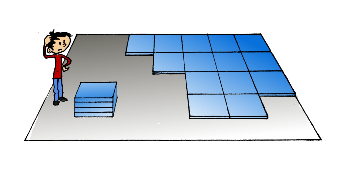
\includegraphics[width=4.8cm]{carrelage}
  \end{minipage} \\
 \begin{enumerate}
  \item La surface rectangulaire mesure 12 cm par 18 cm. Quelle peut être la longueur du côté des carrés ? Y a-t-il plusieurs possibilités ? Que représente(nt) ce(s) nombre(s) pour 12 et 18 ? Mêmes questions lorsque la surface rectangulaire mesure 49 cm par 63 cm, puis 27 cm par 32 cm et enfin 21 cm par 84 cm.
  \item Cherche les dimensions maximales d'un carré pouvant paver une surface rectangulaire de 108 cm par 196 cm.
  \end{enumerate}
\end{partie}

\begin{partie}
Un challenge sportif regroupe 30 filles et 75 garçons. Les organisateurs souhaitent composer des équipes comportant toutes le même nombre de filles et le même nombre de garçons. Comment peux-tu les aider pour qu'ils puissent constituer un nombre maximal d'équipes ? Donne ensuite le nombre de filles et de garçons dans chaque équipe. Explique ta démarche.
\end{partie}

\begin{partie}[PGDC]
\begin{enumerate}
 \item Dresse la liste des diviseurs de 30 et celle des diviseurs de 50. Quel est le plus grand diviseur commun à ces deux nombres ? On appelle ce nombre le \textbf{PGDC} de 30 et 50 et on le note : PGDC $(30 ; 50)$ ou PGDC $(50 ; 30)$.
 \item Quel est le PGDC de 8 et 24 ? Que remarques-tu ? Essaie de formuler une règle à partir de ce que tu as observé.
 \end{enumerate}
\end{partie}

\end{activite}

%%%%%%%%%%%%%%%%%%%%%%%%%%%%%%%%%%%%%%%%%%%%%%%%%%%%%%%%%%%%%%%%%%

\begin{activite}[Multiples communs, PPMC]

\begin{partie}
 \begin{minipage}[c]{0.6\textwidth}
Un engrenage est formé de 2 roues dentées $(A et B)$ qui ont respectivement 8 et 6 dents. Un point $R$ marqué sur une dent de la roue $B$ fait face à un point $S$ marqué entre deux dents consécutives de la roue $A$. On met l'engrenage en mouvement. Après combien de tours de la roue $A$ les points $R$ et $S$ seront-ils pour la première fois à nouveau dans la même position ? Même question lorsque la roue $A$ possède 9 dents et la $B$ 12 dents.
 \end{minipage} \hfill%
 \begin{minipage}[c]{0.2\textwidth}
  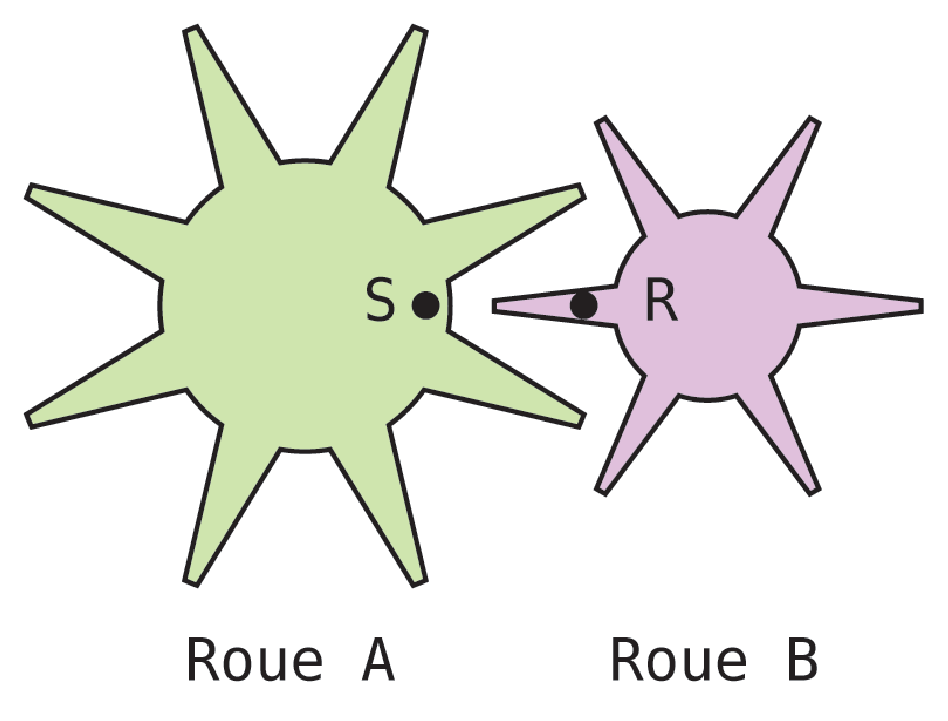
\includegraphics[width=3.8cm]{rouesAB}
  \end{minipage} \\
\end{partie}

\begin{partie}
Pendant l'été, un vendeur de glace ambulant visite le quartier de Jeannette tous les 7 jours et un autre vendeur de glace visite le même quartier tous les 5 jours. Quand les deux vendeurs sont présents le prix des glaces est diminué. Si les deux vendeurs de glaces ont visité le quartier aujourd'hui, quand sera la prochaine fois où le prix des glaces sera diminué ?
\end{partie}

\begin{partie}[PPMC]
\begin{enumerate}
 \item Dresse la liste des multiples de 9 et celle des multiples de 6. Quel est le plus petit multiple commun à ces deux nombres ? On appelle ce nombre le \textbf{PPMC} de 9 et 6 et on le note : PPMC $(9 ; 6)$ ou PPMC $(6 ; 9)$.
 \item Quel est le PPMC de 7 et 21 ? Que remarques-tu ? Essaie de formuler une règle à partir de ce que tu as observé.
 \end{enumerate}
\end{partie}

\end{activite}

%%%%%%%%%%%%%%%%%%%%%%%%%%%%%%%%%%%%%%%%%%%%%%%%%%%%%%%%%%%%%%%%%%

\begin{activite}[Crible d'Eratostène]

 \begin{minipage}[c]{0.6\textwidth}
Ératosthène était un astronome, géographe, philosophe et mathématicien grec (276 – 194 av. J.-C.).
 \end{minipage} \hfill%
 \begin{minipage}[c]{0.2\textwidth}
  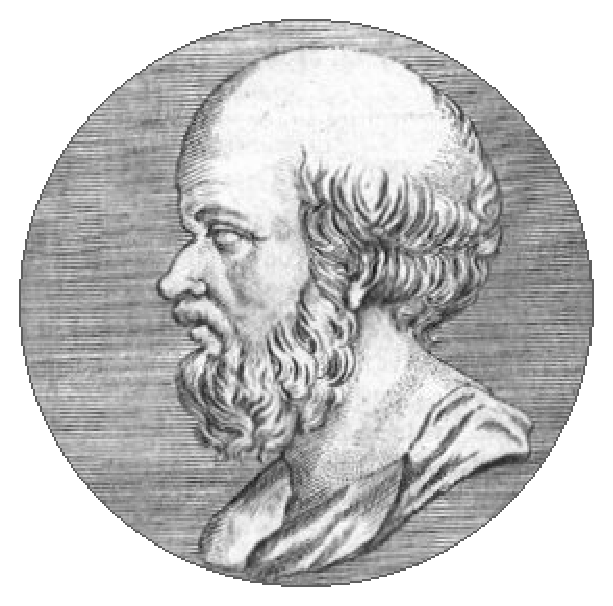
\includegraphics[width=3cm]{monnaie}
  \end{minipage} \\[1em]
  
\begin{tabularx}{1.01\linewidth}{|X|X|X|X|X|X|X|X|X|X|X|X|X|X|X|X|X|X|X|X|}
     \hline
     1 & 2 & 3 & 4 & 5 & 6 & 7 & 8 & 9 & 10 & 11 & 12 & 13 & 14 & 15 & 16 & 17 & 18 & 19 & 20 \\\hline
     21 & 22 & 23 & 24 & 25 & 26 & 27 & 28 & 29 & 30 & 31 & 32 & 33 & 34 & 35 & 36 & 37 & 38 & 39 & 40 \\\hline
     41 & 42 & 43 & 44 & 45 & 46 & 47 & 48 & 49 & 50 & 51 & 52 & 53 & 54 & 55 & 56 & 57 & 58 & 59 & 60 \\\hline
     61 & 62 & 63 & 64 & 65 & 66 & 67 & 68 & 69 & 70 & 71 & 72 & 73 & 74 & 75 & 76 & 77 & 78 & 79 & 80 \\\hline
     81 & 82 & 83 & 84 & 85 & 86 & 87 & 88 & 89 & 90 & 91 & 92 & 93 & 94 & 95 & 96 & 97 & 98 & 99 & 100 \\\hline
  \end{tabularx} \\
  
\begin{enumerate}             
 \item Sur le tableau ci-dessus, entoure le chiffre 2 en rouge et raye tous les multiples de 2 autres que 2. Entoure le chiffre 3 en vert et raye tous les multiples de 3 autres que 3. Recommence avec le premier nombre non rayé et continue le processus jusqu'à ce que tous les nombres soient entourés ou rayés. Utilise des couleurs différentes pour chaque étape.
 \item Quelle est la particularité des nombres entourés ?
 \item Si on applique ce crible à tous les entiers naturels, 163 serait-il entouré ? Et 1\,678\,314 ?
 \item À l'aide du tableau, détermine les diviseurs de 24, 72, 17, 23 et 71.
 \end{enumerate}

\end{activite}

%%%%%%%%%%%%%%%%%%%%%%%%%%%%%%%%%%%%%%%%%%%%%%%%%%%%%%%%%%%%%%%%%%

\begin{activite}[Le triangle de Sierpinski]

\begin{partie}[Répondre avec des 3 et des $\cdot$ uniquement !]

 \begin{minipage}[c]{0.5\linewidth}
La figure de départ est un triangle équilatéral violet. On construit à l'intérieur de celui-ci un triangle bleu obtenu en joignant les milieux des côtés du triangle de départ.
 \end{minipage} \hfill%
 \begin{minipage}[c]{0.4\linewidth}
  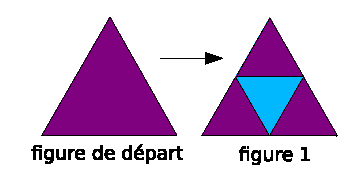
\includegraphics[width=4.9cm]{sierpinski1}
  \end{minipage} \\[1.5em]
 
 \begin{minipage}[c]{0.2\linewidth}
 \begin{center} 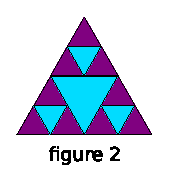
\includegraphics[width=2.2cm]{sierpinski2} \end{center}
 \end{minipage} \hfill%
 \begin{minipage}[c]{0.74\linewidth}
  \begin{enumerate}
   \item De la même façon, on construit un petit triangle bleu dans chacun des triangles violets de la figure 1. Combien obtient-on de triangles violets dans la figure 2 ?
   \item Imaginons que l'on continue à construire des triangles bleus dans les triangles violets. Combien a-t-on de triangles violets dans la figure 4 ? Puis dans la figure 7 (en n'utilisant encore que des 3 et des signes $\cdot$ ) ? Et dans la figure 20 ?
   \end{enumerate}
  \end{minipage} \\[1em]
  
\end{partie}


\begin{partie}[Une nouvelle notation : la notation « puissance »]
La notation « puissance » est utilisée pour remplacer des produits comme dans les exemples suivants :
\begin{itemize}
 \item $9 = \stackrel{2 facteurs}{\overbrace{3 \cdot 3}} = 3^2$ qui se lit « 3 au carré » ou « 3 puissance 2 » ou « 3 exposant 2 » ;
 \item $81 = \stackrel{4 facteurs}{\overbrace{3 \cdot 3 \cdot 3 \cdot 3}} = 3^4$ qui se lit « 3 puissance 4 » ou « 3 exposant 4 ».
 \end{itemize}
\begin{enumerate}
 \item Écris, à l'aide de la notation « puissance », le nombre de triangles violets qu'il y a dans la figure 7 puis calcule ce nombre. Recommence pour la figure 20.
 \item À l'aide de ta calculatrice, indique combien il y a de triangles violets dans la figure 13, la figure 18, la figure 10 et enfin dans la figure 15. Existe-t-il un moyen d'effectuer ces calculs facilement avec ta calculatrice ?
 \end{enumerate}
\end{partie}

\end{activite}

%%%%%%%%%%%%%%%%%%%%%%%%%%%%%%%%%%%%%%%%%%%%%%%%%%%%%%%%%%%%%%%%%%

\begin{activite}[Des produits avec 2, 3 et 5]

Nous allons exprimer certains nombres sous la forme de produits. Dans cette activité, les seuls facteurs autorisés sont : 2 ; 3 et 5. Nous utiliserons la notation « puissance » dès que cela est possible.\\[0.25em]

 \begin{minipage}[t]{0.1\linewidth}
 \underline{Exemples} : 
  \end{minipage} \hfill%
 \begin{minipage}[t]{0.86\linewidth}
$25 = 5 \cdot 5$ peut s'écrire $25 = 5^2$ ;

$48 = 2 \cdot 2 \cdot 2 \cdot 2 \cdot 3$ peut s'écrire $48 = 2^4 \cdot 3$ ;

$90 = 2 \cdot 3 \cdot 3 \cdot 5$ peut s'écrire $90 = 2 \cdot 3^2 \cdot 5$.
 \end{minipage} \\

\begin{enumerate}
 \item Exprime de la même façon les nombres 4 ; 12 ; 27 ; 30 ; 45 et 108. Peut-on exprimer le nombre 26 de la même façon ? Justifie. \label{MbsEntMultDivis_acti1}
 \item Un élève a écrit l'égalité suivante : $54 = 2^1 \cdot 3^3$. En considérant que sa réponse est bonne, combien vaut $2^1$ ?
 \item Un élève a écrit l'égalité suivante : $50 = 2^1 \cdot 3^0 \cdot 5^2$. En considérant que sa réponse est bonne, combien vaut $3^0$ ?
 \item Réécris les trois exemples du départ puis les nombres de la question \ref{MbsEntMultDivis_acti1} sous la forme  $2^a \cdot 3^b \cdot 5^c$ (a, b et c sont des entiers naturels, éventuellement égaux à 0 ou 1).
 \item Trouve le plus possible de nombres inférieurs à 100 qui peuvent s'exprimer sous la forme d'un produit ne comportant que des 2, des 3 et des 5.
 \item Si maintenant les facteurs autorisés sont tous les nombres premiers. Exprime sous la forme d'un produit de facteurs premiers les nombres 42, 66, 198 et 990.
 \end{enumerate}
 
\end{activite}
